\subsection{Boundary conditions at corner ghost points}
\newcommand{\dr}{{\Delta r}}
\newcommand{\ds}{{\Delta s}}


Using Taylor series as the corner point $u(-1,-1)$ in two-dimensions gives
\begin{eqnarray*}
  u(+1,+1) &=& u(0,0) +\dr~u_r + \ds~u_s + \dr^2/2~ u_{rr} + \dr \ds~ u_{rs} + \ds^2/2~ u_{ss} + \ldots \\
  u(-1,-1) &=& u(0,0) -\dr~u_r - \ds~u_s + \dr^2/2~ u_{rr} + \dr \ds~ u_{rs} + \ds^2/2~ u_{ss} + \ldots 
\end{eqnarray*}
Combining these equations gives
\[
  u(-1,-1) = u(1,1) -2 \dr~u_r -2 \ds~u_s + O(\max(\dr,\ds)^3)
\]
and using the approximations
\begin{eqnarray*}
  u_r &=& (u(1,0)-u(-1,0))/(2 \dr) + O(\dr^2) \\
  u_s &=& (u(0,1)-u(0,-1))/(2 \ds) + O(\ds^2)
\end{eqnarray*}
to give the following approximation that we use at corners.
\begin{equation}
   u(-1,-1) \approx u(1,1) -( u(1,0)-u(-1,0) ) - (u(0,1)-u(0,-1)) \label{eq:corner}
\end{equation}
The boundary condition~(\ref{eq:corner}) will reduce to a symmetry boundary condition
if the neighbouring points also satisfy the symmetry condition.



Now consider developing higher order approximations for corner points.

\newcommand{\ra}{{r_1}}
\newcommand{\rb}{{r_2}}
\newcommand{\rc}{{r_3}}
\newcommand{\dra}{{\Delta r_1}}
\newcommand{\drb}{{\Delta r_2}}
\newcommand{\drc}{{\Delta r_3}}
\newcommand{\trunc}{O(|\rv|^6)}
\newcommand{\Ds}{{\cal D}}

By Taylor series,
\begin{align}
  u(\pm\ra,\pm\rb,\pm\rc)&= u(0,0,0) \pm \Ds_1(\ra,\rb,\rc) + \Ds_2(\ra,\rb,\rc) 
                            \pm \Ds_3(\ra,\rb,\rc) + \Ds_4(\ra,\rb,\rc) + \trunc \label{eq:taylor3d}
\end{align}
where
\begin{align*}
  \Ds_1(\ra,\rb,\rc) &= \Big(\ra \partial_\ra + \rb \partial_\rb + \rc\partial_\rc \Big) u(0,0,0) \\
  \Ds_2(\ra,\rb,\rc) &= {1\over2}\Big( \ra^2\partial_\ra^2+ \rb^2\partial_\rb^2+ \rc^2\partial_\rc^2
      +2\ra \rb\partial_\ra\partial_\rb + 2\ra \rc\partial_\ra\partial_\rc +2\rb \rc\partial_\rb\partial_\rc 
                       \Big)u(0,0,0)  \\
  \Ds_3(\ra,\rb,\rc) &= {1\over3!}\sum_{m_1=1}^3\sum_{m_2=1}^3\sum_{m_3=1}^3
                         r_{m_1} r_{m_2} r_{m_3} \partial_{m_1}\partial_{m_2}\partial_{m_3} u(0,0,0) \\
                     &={1\over3!}\Big( \ra^3\partial_r^3+ \rb^3\partial_\rb^3+ \rc^3\partial_\rc^3
   +3 \ra^2 \rb\partial_\ra^2\partial_\rb + 3 \ra\rb^2\partial_\ra\partial_\rb^2  \\
  &~~~~ +3 \ra^2 \rc\partial_\ra^2\partial_\rc + 3 \ra\rc^2\partial_\ra\partial_\rc^2 
   +3 \rb^2 \rc\partial_\rb^2\partial_\rc+ 3 \rb\rc^2\partial_\rb\partial_\rc^2 \\
  &~~~~ +6 \ra\rb\rc \partial_\ra\partial_\rb\partial_\rc  \Big) u(0,0,0)  
\end{align*}


For Neumann type boundary conditions which correspond to even functions at the boundary (the homogeneous
Poisson problem will have all odd derivatives zero at the boundary) we wish to eliminate the 
even derivatives from the Taylor expansion for $u(-\ra,-\rb,-\rc)$. From equation~\ref{eq:taylor3d} we form
\[
 u(\ra,\rb,\rc)-u(-\ra,-\rb,-\rc)= 2\Ds_1(\ra,\rb,\rc)+2\Ds_3(\ra,\rb,\rc)+ \trunc
\]
We use the approximations
\begin{align*}
  \partial_\ra u(0,0,0) &\approx \Ds_{\ra} u(0,0,0) \\
                        &\equiv D_{0\ra}(1-{1\over 6} \Delta_{+\ra}\Delta_{-\ra}) u(0,0,0) + O(\dra^4) \\
  \partial_\ra^3 u(0,0,0) &\approx \Ds_{\ra}^{(3)} u(0,0,0) \\
                        &\equiv  D_{0\ra}D_{+\ra}D_{-\ra} u(0,0,0) + O(\dra^2) \\
  \partial_\ra\partial_\rb^2 u(0,0,0) &\approx \Ds_{\ra,\rb^2}^{(3)} u(0,0,0)\\
                        &\equiv  D_{0\ra}D_{\pm\rb}^2 u(0,0,0) + O(\dra^2+\drb) \\
  \partial_\ra\partial_\rb\partial_\rc u(0,0,0) &\approx \Ds_{\ra,\rb,\rc} \\
                        &\equiv D_{0\ra}D_{0\rb}D_{0\rc} u(0,0,0)+O(\Delta r^2)
\end{align*}
where the sign of the one-sided difference approximation to the second derivative in
$D_{0\ra}D_{\pm\rb}^2 u(0,0,0)$ should be chosen so the stencil extends away from the ghost point.
This one-sided difference is needed to avoid coupling the ghost point. The centred difference for
the first derivative portion of $D_{0\ra}D_{\pm\rb}^2 u(0,0,0)$ is needed so that the formula
reduces to an even symmetry condition for even functions.

Whence we are led to the approximation
\begin{align}
u(-\ra,-\rb,-\rc)&= u(\ra,\rb,\rc) - 2\Big\{ \ra \Ds_{\ra} + \rb \Ds_{\rb} + \rc \Ds_{\rc}\Big\} u(0,0,0) \nonumber \\
    &-  {2\over3!}\Big\{ \ra^3 \Ds_{\ra}^{(3)} + \rb^2 \Ds_{\rb}^{(3)} + \rc^3 \Ds_{\rc}^{(3)} \nonumber\\
    &~~~~          +3\Big( \ra^2\rb \Ds_{\rb,\ra^2}^{(3)} + \ra\rb^2 \Ds_{\ra,\rb^2}^{(3)} + \ldots \Big) \nonumber\\
    &~~~~   + 6 \ra\rb\rc \Ds_{\ra,\rb,\rc}
                  \Big\} u(0,0,0) + O(\Delta r^4) \label{eq:cornerbc4}
\end{align}
Equation~(\ref{eq:cornerbc4}) can be used to determine $u$ at ghost points along edges such as
$u(-\dra,-\drb,0)$, $u(-\dra,0,-\drc)$, $u(-2\dra,\drb,0)$ and corners such as $u(-\dra,-\drb,-\drc)$ and
$u(-2\dra,-2\drb,-\drc)$. Note that in the case for $u(-\dra,-\drb,-\drc)$, this value appears 
in the expression for $\Ds_{\ra,\rb,\rc}$ in the right-hand-side
of (\ref{eq:cornerbc4}) and thus one must solve for this value.

For even functions, $u(x,y,z)=u(-x,-y,-z)$, this approximation will reduce to the even-symmetry 
condition
\[ 
   u(-\dra,-\drb,-\drc)= u(\dra,\drb,\drc)
\]
This is the property we desire for edges and corners that are adjacent to faces with Neumann boundary conditions.


Here is an example of the fourth order boundary condition, equation~(\ref{eq:cornerbc4}),
 for $\ra=\dra$, $\rb=\drb$ and  $\rc=0$
\begin{align*}
u_{i_1-1,i_2-1,i_3} &=(-3u_{i_1+1,i_2,i_3}+3u_{i_1-1,i_2,i_3} +u_{i_1+2,i_2-1,i_3} -u_{i_1+2,i_2+1,i_3} \\
       &  ~~~~~ +6u_{i_1+1,i_2+1,i_3} -2u_{i_1+1,i_2-1,i_3}-2u_{i_1-1,i_2+1,i_3}  \\
       &  ~~~~~ -3u_{i_1,i_2+1,i_3}+3u_{i_1,i_2-1,i_3}
          +u_{i_1-1,i_2+2,i_3}-u_{i_1+1,i_2+2,i_3} )/2
\end{align*}

Figure~(\ref{fig:fourthOrderCornerBC}) presents some results using these corner boundary conditions.
The results show that the convergence rate is improved over the results obtained using an extrapolation
boundary condition.

\renewcommand{\figWidth}{.495\linewidth}
\begin{figure}
\begin{center}
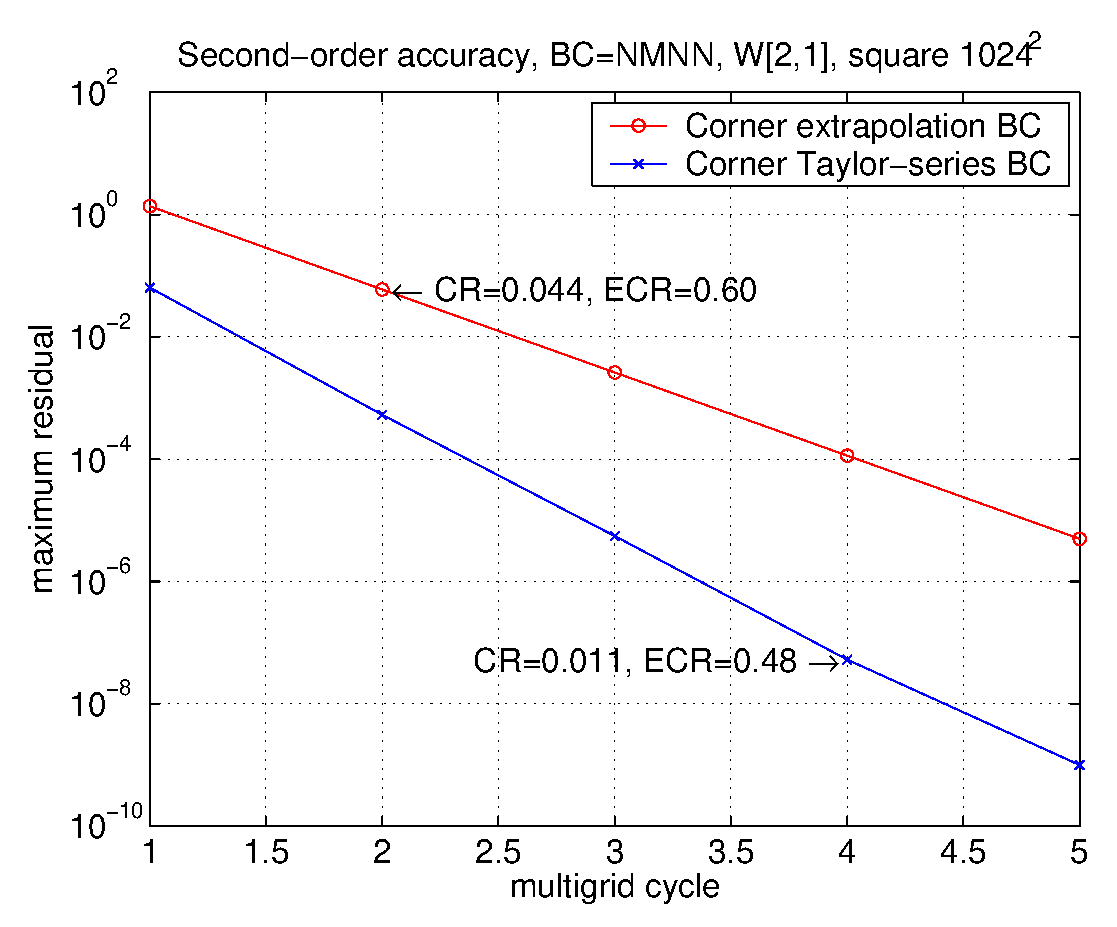
\epsfig{file=\ogmgDir/secondOrderCornerBC.square1024.eps,width=\figWidth}
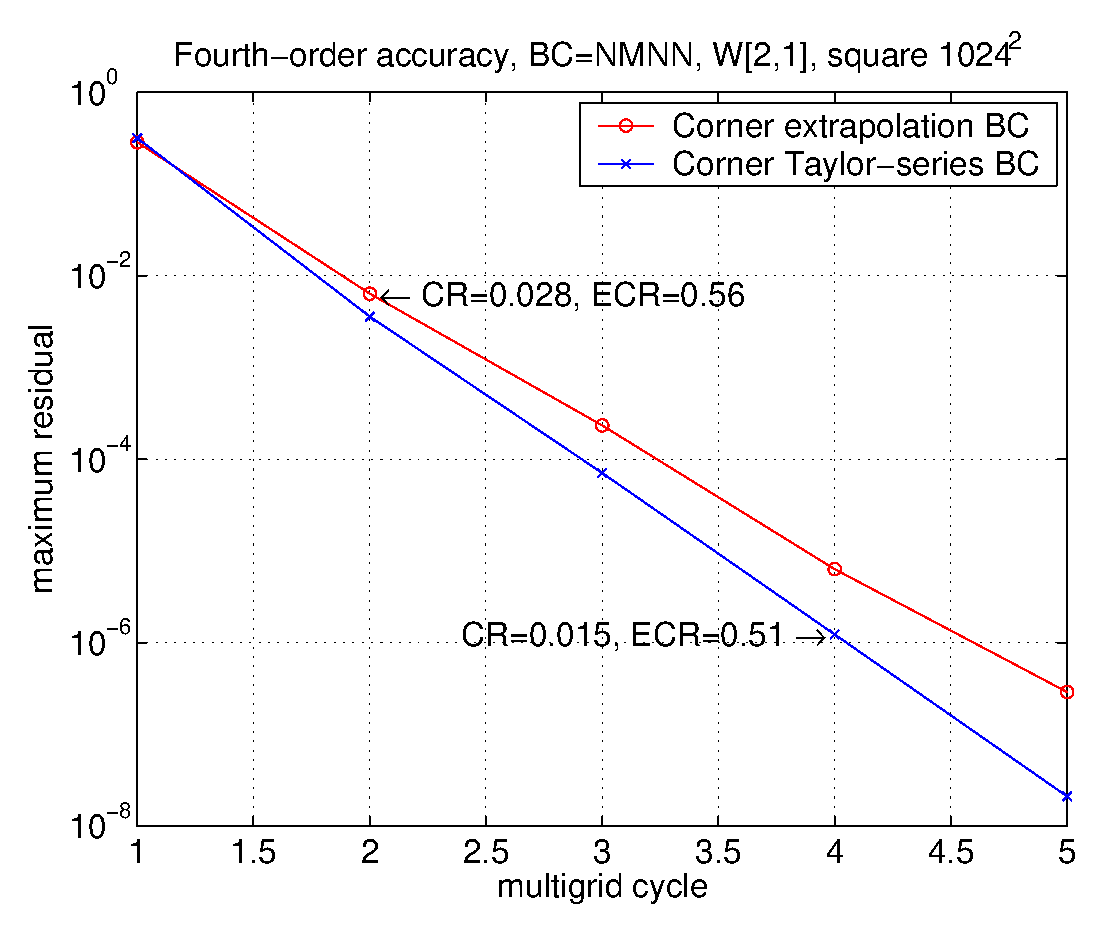
\epsfig{file=\ogmgDir/fourthOrderCornerBC.square1024.eps,width=\figWidth}
\end{center}
\caption{A comparison of two corner ghost point boundary conditions.
The boundary conditions for the square were Neumann on three sides and a mixed condition on the fourth side.
Results are shown for a W[2,1] cycle. The {\em Taylor-series} boundary condition that reduces to an
even-symmetry condition performs
better than extrapolation. }
\label{fig:fourthOrderCornerBC}
\end{figure}